\documentclass[11pt, twocolumn]{article}

\usepackage[utf8]{inputenc}
\usepackage{graphicx}
\usepackage{amsmath}
\usepackage[a4paper, total={7in, 9in}]{geometry}
\usepackage[colorlinks]{hyperref}
\usepackage{siunitx}
\usepackage{amsmath}
\title{Statistics Intuition Cheatsheet}
\author{Yahya~Almardeny\\almardeny@gmail.com}
\date{September 2019}

\begin{document}
\begin{titlepage}
\maketitle
\end{titlepage}
\section{Abstract}
The purpose of this sheet is to provide a quick recap about the {\color{blue} intuition} of the fundamental concepts in statistics and/or its {\color{blue} applications}.\\
It assumes that you are familiar with the formulas of the basic statistical tests.\\
This sheet is {\color{red} not} about how to calculate tests or solve statistical issues.
\section{Descriptive Statistics}
\begin{itemize}
\item \textbf{Mean ($\mu$)}: The Arithmetic Average of Data Values. It is highly susceptible to extreme values (i.e. outliers).
\begin{itemize}
\item \textit{Example 1 - No Outliers}:\\ 
$Data = [1,2,3,4,5] \implies \mu = 3$  which makes sense since 3 is within the range [1-5] (i.e. good representative of the data center).
\item \textit{Example 2 - With Outliers}:\\
$Data = [1,2,3,4,5, {\color{red} 50}] \implies \mu = 10.83$  which is not a perfect representative of the center of data since 10.83 is outside the range [1-5] that contains the {\color{blue} majority} of data points, rather the mean moved towards the value 50!.
\end{itemize}
\end{itemize}

\begin{itemize}
\item \textbf{Median}: The Middle Number in an Ordered Array. It is \textbf{not} affected so much by outliers.
\begin{itemize}
\item \textit{Example 1 - No Outliers}:\\ 
$Data = [1,2,3,4,5] \implies median = 3$  note how it is the same as the mean value above because the distribution of the data points is {\color{blue} perfectly symmetric} and has {\color{blue} zero skewness}.
\item \textit{Example 2 - With Outliers}:\\
$Data = [1,2,3,4,5, {\color{red} 50}] \implies median = 3.5$  which is {\color{blue} still a good} representative of the center of data unlike the mean that we got above 10.83!.
\end{itemize}
\end{itemize}

\begin{itemize}
\item \textbf{Quartiles}: Values that divide an ordered list of numbers into quarters Q1, Q2 (the median), and Q3. It is mainly used to find Interquartile (see next) and in the Box and Whisker Plot which can describe the center and {\color{blue} spread} of the distribution visually in a five-number summary. Ponder the following Box plots (On left: Data=[1,2,3,4,5,6], On right: Data=[1,2,3,4,50,60] which is skewed):\\\\
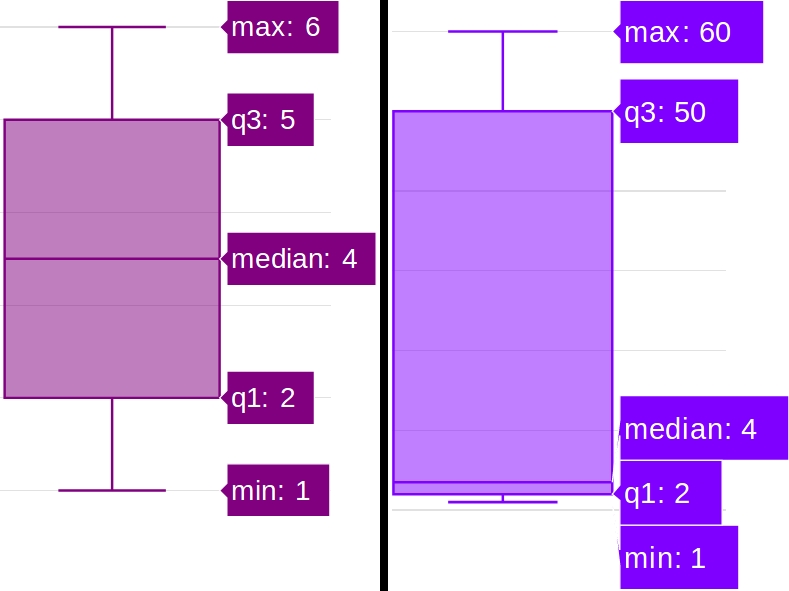
\includegraphics[width=\linewidth,keepaspectratio]{figs/quartiles.jpeg}
\end{itemize}

\begin{itemize}
\item \textbf{Interquartile (IQR)}: It is Q3 - Q1. However, it is not used that much. It can be used to reflect the degree of the outlierness cutoff.
\begin{itemize}
\item \textit{Example}:\\ 
Consider the following 3 data samples:

$Data_1 = [1,2,3,4,5] ~~ Q1=2, ~~ Q3=5 \implies IQR_1 = 3$  \\
$Data_2 = [1,2,3,4,{\color{red} 50}] ~~ Q1=2, ~~ Q3=16 \implies IQR_2 = 14$  \\
$Data_3 = [1,2,3,4,{\color{red} 100}] ~~ Q1=2, ~~ Q3=28 \implies IQR_3 = 26$  \\
note how $IQR_3 > IQR_2$ because $Data_3$ contains more extreme element than $Data_2$: $100 > 50$.
\end{itemize}
\end{itemize}

\begin{itemize}
\item \textbf{Range}: It is the difference between the largest and smallest values in a dataset. It provides an indication of statistical dispersion and it is most useful in representing the dispersion of small data sets. It can be used as a reference to trigger a warning if readings are not within the acceptable range. However, it is very sensitive to outliers that could lead to a misleading result.
\end{itemize}

\begin{itemize}
\item \textbf{Standard Deviation ($\sigma$)}: Describes how Data Points Vary/Spread around the Mean (i.e. the variability of data). It is highly affected by outliers and it is not a perfect measure for finance risk (see later). It has very important uses, such as in Variance, Z-Score and Coefficient of Variation (CV) (see later).
\end{itemize}

\begin{itemize}
\item \textbf{Variance ($\sigma^2$)}: The $\sigma$ Squared (i.e. the average distance from the mean squared). Its importance (over $\sigma$) comes from its {\color{blue} mathematical properties}. For example: Let $X, ~ Y$ be two independent random variables. Then mathematically, we can find the Variance of the two variables like this: $\sigma^2(X \pm Y) = \sigma^2(X) + \sigma^2(Y)$. However, $\sigma$ fails to find: $\sigma(X + Y) = \sqrt{\sigma^2(X) + \sigma^2(Y)} = \sqrt{\sigma(X)^2 + \sigma(Y)^2}$ which is not $\sigma(X) + \sigma(Y)$.
\end{itemize}


\begin{itemize}
\item \textbf{Z-Score}: (a.k.a  standard score). It is the number of standard deviations from the mean a data point is. In other words, the Z-score of a data point, is the distance between that point and the mean {\color{blue}normalized} by the standard deviation: $Z = \frac{x - \mu}{\sigma} $
\begin{itemize}
\item \textit{Its Importance - Example}:\\
Let $X, ~Y$ be two samples of students' grades in Maths from two different schools. Let $\mu_x = 70,~ \sigma_x = 15$, $\mu_y = 70,~ \sigma_x = 5$. Now if you know that Sarah from School $X$  scored 80 in Maths, and Omar from School $Y$ scored 75 in Maths. Whose grade (i.e. rank) is better in their school? You might think at the beginning it is Sarah. However, to do the comparison, we need to compare Apples to Apples, and since $\sigma_x \neq \sigma_y \implies$  we normalize by converting their grades to Z-Scores:\\
$Z_{sarah} = \frac{80 - 70}{15} = 0.66$ and $Z_{omar} = \frac{75 - 70}{5} = 1$. \\It turned out that Omar is farer from the mean in his school compared to Sarah. Thus Omar's rank is higher in {\color{blue} his} school compared to Sarah in {\color{blue} her} school!.
\end{itemize}
\end{itemize}


\begin{itemize}
\item \textbf{Finance Risk and Coefficient of Variation (CV)}:  
The finance risk concerns about the danger or possibility that investors will lose money. If we take the return as an example, the finance risk would concern about the variation of return values over the years. Thus, the higher the standard deviation, the higher the risk (i.e. the return is not so consistent and it fluctuates a lot). However, $\sigma$ is not the best measure since it doesn't take the mean of the returns into account as it is shown in the following example.
\begin{itemize}
\item \textit{Example}:\\
Suppose that you have two datasets about the yearly rate of return of two Stocks $A$ and $B$ during the past 5 years: \\
$Stock_A = [22\%, 15\%, 20\%, 26\%, 15\%]$ \\
$Stock_B = [8\%, 10\%, 12\%, 14\%, 16\%]$ \\
Calculations show that $\sigma_{stock_A} = 4.27$ and  $\sigma_{stock_B} = 3.16$ which indicates that $Stock_A$ is more risky than $Stock_B$. 
Nevertheless, $CV_{stock_A} = 24.09$ and  $CV_{stock_B} = 26.35$ which indicates that $Stock_B$ is more risky than $Stock_A$, and that's more reliable result. That's because the Coefficient of Variation $CV = \frac{\sigma}{\mu}$ adjusts for the size of the project and puts the standard deviation into {\color{blue} context}. Also, it is {\color{blue} safer} when you have huge difference in the means and want to compare their variations (you can think about it as a "relative $\sigma$" or a "normalized $\sigma$").
\end{itemize}
\end{itemize}

\begin{itemize}
\item \textbf{Linear Transformation}:  
Intuitively, when we apply linear transformation on a dataset, we basically change the center and the spread of data by Adding or/and Subtracting or/and Multiplying by or/and
Dividing by a {\color{blue} constant}.\\
Note that Linear Transformation does {\color{red} not} change the relationship between the variables (e.g. the correlation still the same), rather the mean is shifted and the variance is scaled.\\
One example you've already seen is the Z-Score where we normalized by $\sigma$ to make new data has mean 0 and variance 1.\\
Linear transformation helps to get rid of skewness in data, for example, Logarithm Transformation reduces right skewness, where Square Transformation reduces Left Skewness.


\end{itemize}

\begin{itemize}
\item \textbf{Empirical Rule}:
There is a trend found in data that strictly has a mound shape. That trend called the Empirical Rule (or the 68–95–99.7 rule), which says: 
 68.27\% of the data falls within 1 standard deviation.
 95.45\% falls within $2\sigma$ 
 and 99.73\% falls within $3\sigma$ from the mean.
 That's useful when you know only the mean and the standard deviation.
\end{itemize}

\begin{itemize}
\item \textbf{Chebyshev's Rule}:
It is an alternative to the Empirical Rule when you {\color{red} do not} have a bell-shaped data (i.e. data is skewed).\\
The rule says: {\color{blue} at least} 0\% of data is within $1\sigma$, {\color{blue} at least} 75\% of data is within $2\sigma$, {\color{blue} at least} 89\% of data is within $3\sigma$.
\end{itemize}

\begin{itemize}
\item \textbf{Skewness}:
It measures the degree of asymmetry exhibited by data.\\ As a rule of thumb: Negative Values = Skewed Left, Positive Values = Skewed Right, If $|skewness| < 0.8 \implies$ Don't need to transform data.
\end{itemize}

\begin{itemize}
\item \textbf{Covariance}:
It measures the joint {\color{blue}variability} of two random variables. Intuitively, it is similar to Variance, but this describes how {\color{blue}two} variables vary {\color{blue}together}. Covariance reflects the trend (relationship) between the two variables (Positive, Negative, or No Relationship) which has enormous applications.
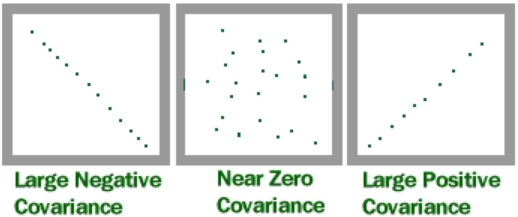
\includegraphics[width=\linewidth,keepaspectratio]{figs/covariance.jpeg}

\end{itemize}

\begin{itemize}
\item \textbf{Covariance Matrix}:
Intuitively, it is a matrix that generalizes the notion of variance to multiple dimensions. It calculates (and therefor find if there's a relationship) for every combination of variables.
It has a lot of applications, such in Principle Component Analysis, Cholesky Decomposition and fixing Model Overfitting (we look at the features that have similar / very high covariance and we remove one of each since they are redundant - see next example).
\begin{itemize}
\item \textit{Example of Redundant Variables}:
\[ Let ~~ S =
\begin{bmatrix}
	A & B & C\\
    1 & 3 & 6 \\
    4 & -4 & -8 \\
    10 & 1 & 2\\
    5 & 20 & 40\\
    7 & 28 & 56\\
\end{bmatrix} \in \rm I\!R^3
\]
be a dataset. Here we have 3 features (i.e. variable per column, name them A, B and C from left to right respectively). At a glance, you can see that variable C is always double the value of B (which is redundant in modeling). Now, suppose that we have a really big dataset, it will be impossible to analyze it by just looking at it. Thus, we can use the Covariance Matrix which reflects how feature C is related to feature B (it has high covariance highlighted in red):
\[ Cov. ~ Matrix =
\begin{bmatrix}
	& A & B & C\\
    A & 11.3 & 8.45 & 16.9 \\
    B & 8.45 & 187.3 & {\color{red} 374.6} \\
    C & 16.9 & {\color{red} 374.6} & 749.2\\
\end{bmatrix}
\]
\end{itemize}
\end{itemize}

\begin{itemize}
\item \textbf{Correlation}:
Very similar to Covariance. Correlation measures the {\color{blue}strength} of the dependence or association between two variables and its {\color{blue}direction}. You can think about it as a "custom" relationship and it has a lot of applications, for example but not limited to:
\begin{itemize}
 \item Finding the influence of the price on the quantity of the product.
 \item Checking for Multicollinearity between features before applying Multiple Linear Regression or when calculating the variance inflation factor (VIF)).
 \end{itemize}
Correlation ranges only between -1 and 1 (unlike Covariance) and it has 3 main types:
\begin{itemize}
\item \textit{Pearson r Correlation}:
The most popular coefficient. It measures the strength of a {\color{blue}linear} relationship between two variables (both variables should be normally distributed and have homoscedasticity).\\
According to Cohen's Standards, its \textit{absolute} value has overall 3 categories:
\begin{itemize}
  \item Weak: up to 0.29
  \item Medium: 0.3 to 0.49
  \item Strong: 0.5 and above
\end{itemize}
\end{itemize}

\begin{itemize}
\item \textit{Spearman Rank Correlation}:
It measures the strength of a {\color{blue}monotonic} relationship between two variables. A monotonic relationship is where one variable increases, the other increases or decreases but not linearly. Ponder the following graph:
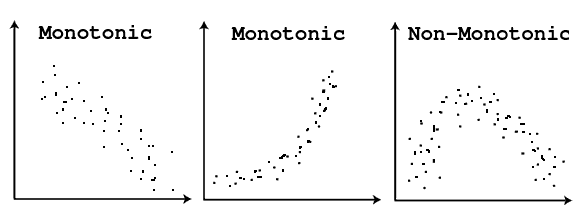
\includegraphics[width=\linewidth,keepaspectratio]{figs/monotonic.png}
\end{itemize}

\begin{itemize}
\item \textit{Kendall Rank Correlation}:
It represents a {\color{blue}probability}; that is the difference between the probability that the two variables are in the same order versus the probability that the two variables are in different orders.\\
It is very similar to Spearman Rank Correlation, because both are for Rank Correlation and the interpretations of both coefficients are very similar and thus invariably lead to the same inferences. However, Kendall Correlation is recommended to be used with {\color{blue}smaller sample sizes} since P-values are more accurate and less sensitive to error.
\end{itemize}
\end{itemize}




\section{Probability}
\begin{itemize}
\item \textbf{Definition}: Provides measures for reasoning the likelihood that an event will occur in an experiment (measure of uncertainty).
\end{itemize}
\begin{itemize}
\item \textbf{Rule}: The probability of each outcome $s$ of any Event, should satisfy:
\begin{itemize}
\item within the range [0 - 1]: $ 0 \leq P(s) \leq 1$.
\item all probabilities should sum up to 1 $\Sigma P(s_i) = 1$
\item the complement rule: $P(s) = 1 - P(\bar{s})$ : the probability of $s$ to happen equals the 1 - the probability of $s$ doesn't happen.
\end{itemize}
\end{itemize}
\begin{itemize}
\item \textbf{Probability of Events:}
\begin{enumerate}
\item \textbf{Marginal probability}: Simply $P(A)$ which means {\color{blue} unconditional probability}.
\item \textbf{Addition Rule}: $P(A \cup B) = P(A) + P(B) - P(A \cap B)$ where $\cup$ means OR, $\cap$ means AND. Note how we are {\color{blue}adding up} probabilities because we want the probability of A {\color{blue}OR} B to happen, and that should intuitively {\color{blue}increase} the overall chances.
\item \textbf{Joint (Compound) Probability Rule}:
	\begin{enumerate}
	\item Independent Events: $P(A \cap B) = P(A) \times P(B)$.
	\item Dependent Events: $P(A \cap B) = P(A) \times P(B | A)$. where $P(B | A)$ reads: Probability of B given A had happened.
	\end{enumerate}
	Note how we {\color{blue}multiply} here, so the result will be {\color{blue}lesser} than any of P(A) and P(B) because we are working with numbers between 0 and 1. That makes sense because intuitively the overall chances should {\color{blue}decrease} since we want both A {\color{blue}AND} B to happen.
\item \textbf{Conditional Probability}: $P(A | B) = \frac{P(A \cap B)}{P(B)}$
\item \textbf{Bayes Theorem}: $P(A | B) = \frac{P(B | A) \times P(A)}{P(B)}$. It gives the probability of A based on prior knowledge of B.
\end{enumerate}
\end{itemize}

\begin{itemize}
\item \textbf{Probability Distributions:}
\begin{enumerate}
\item \textbf{Probability Mass Function (PMF)}: Gives the probability a {\color{blue}discrete} random variable $X$ takes on the value $x$: $P( X = x)$.
\begin{figure}[h!]
  \centering
  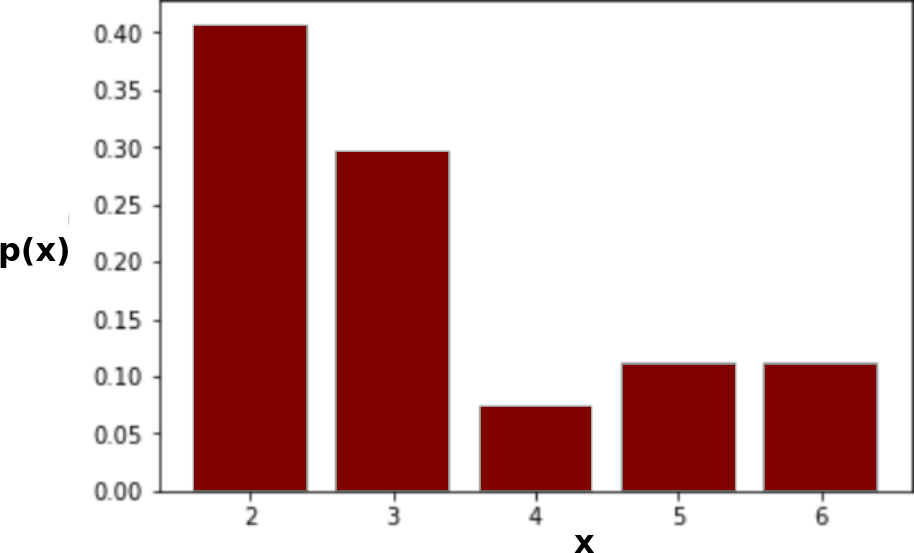
\includegraphics[width=0.75\linewidth]{figs/PMF.png}
\end{figure}
\item \textbf{Probability Density Function (PDF)}: Gives the probability a {\color{blue}continuous} random variable $X$ takes on the value $x$: $P( X = x)$ which means {\color{blue}how dense} the probability of $X$ near $x$, and it will be the definite Integrals between two points.
\begin{figure}[h!]
  \centering
  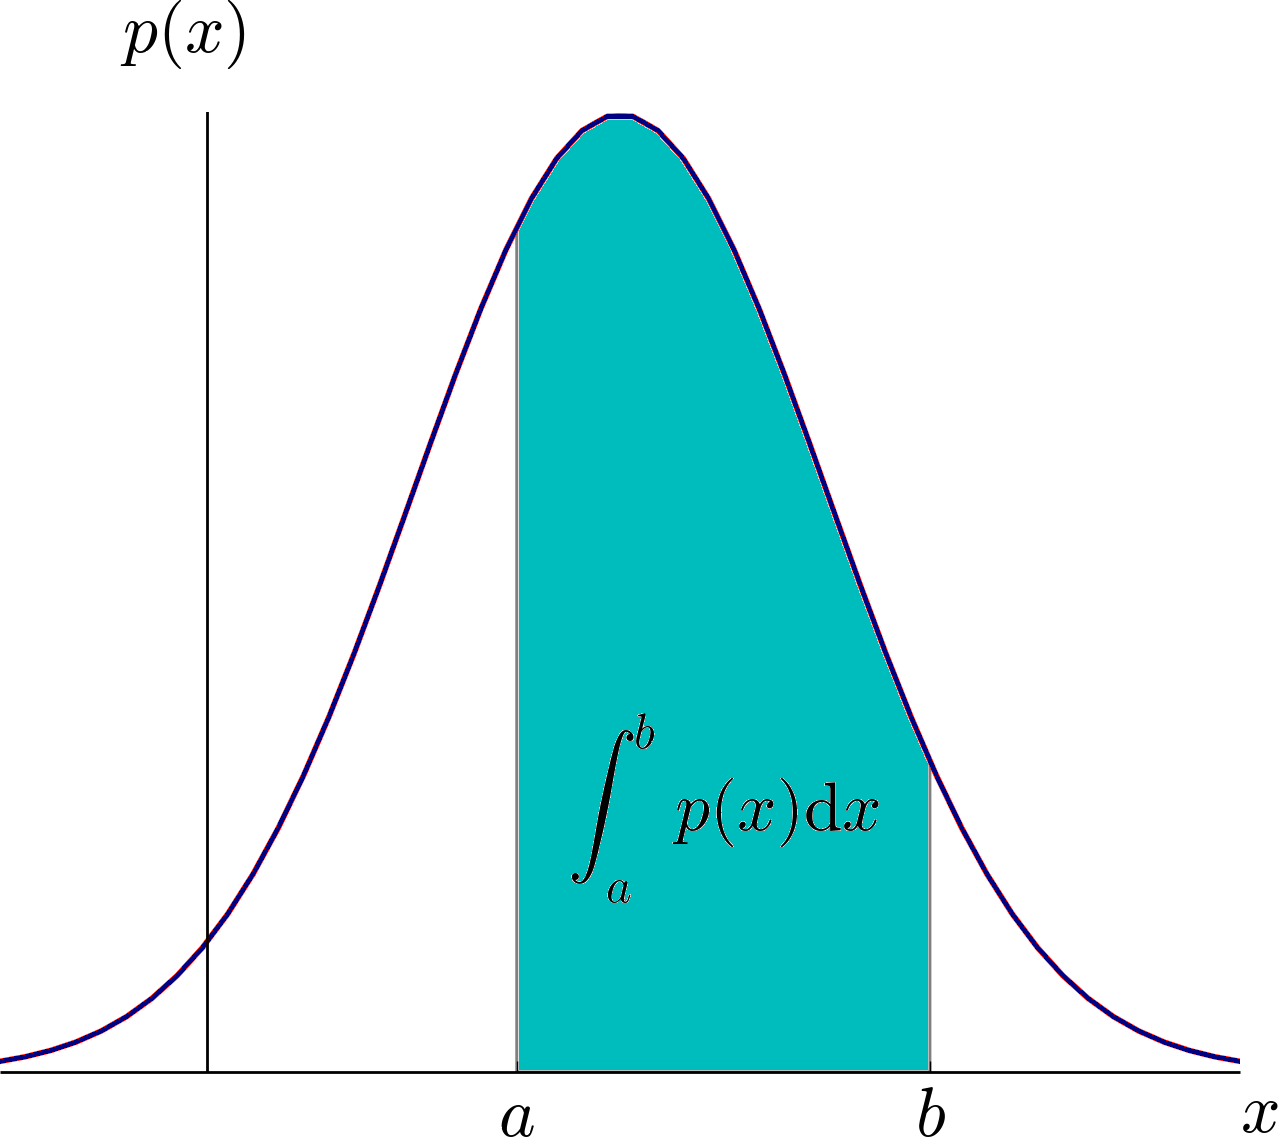
\includegraphics[width=0.65\linewidth]{figs/PDF.png}
\end{figure}
\item \textbf{Cumulative Density Function (CDF)}: Gives the probability a random variable $X$ is less than or equals the value $x$: $P( X \leq x)$. It is  cumulative because it adds the probabilities up to $x$.
	\begin{enumerate}
	\item For Discrete R.V: It is the summation of previous probabilities $\Sigma p(x_i)$.
	\item For Continuous R.V: It is the integral $\int_{-\infty}^{x} p(x) dx$
	\end{enumerate}
\end{enumerate}
\end{itemize}


\begin{itemize}
\item \textbf{Expected Value of Random Variable:}
Intuitively, it is the long-run average value of repetitions of the same experiment it represents (i.e. what outcome to expect on long run, you can think about it as the "mean")
\begin{enumerate}
\item \textbf{For a Discrete R.V}: It is the average of R.V values based on their associated probabilities $E(X) = \Sigma (x_i \times p(x_i))$.
\item \textbf{For a Continuous R.V}: $E(X) = \int_{-\infty}^{\infty} x f(x) dx$ where $f(x)$ is probability density function.
\end{enumerate}
\end{itemize}


\begin{itemize}
\item \textbf{The Law of Large Numbers:}
Let $X$ be R.V of a population where its expected value (i.e Mean) is $E(X)$. Let $\overline{X_n} = \frac{x_1 + x_2 + ... x_n}{n}$ be the mean of $n$ {\color{blue}samples} $\in X$. As $n \to \infty$ : $\overline{X_n} \to E(X)$. That means as we do more experiments, the practical outcomes become {\color{blue} closer and closer} to the outcomes of the probability theory.
\end{itemize}

\begin{itemize}
\item \textbf{Statistical Distributions}\footnote{It is a big long topic, the purpose here is to create your map of knowledge, so you can associate each distribution with a few words. Only the most popular distributions included here.}
\begin{enumerate}
\item \textbf{Binomial Distribution}:
\begin{itemize}
\item How many success in finite number of trials
\item Keywords: {\color{blue} Fixed and Independent} Trials.	
\item \textit{10\% Rule}: we assume independence (where it should be applied) if the sample $\leq$ 10\% of the population.
\item The more trials we do, the more Binomial becomes Normal distribution.
\end{itemize} 

\item \textbf{Bernoulli Distribution}: Simply a Binomial Distribution with just {\color{blue} one} trial. 
\item \textbf{Geometric Distribution}: 
\begin{itemize}
\item  Keywords: {\color{blue} How many trials until success?}.
\item  It is similar to Binomial dist. but here we do not have fixed number of trials because we do not know ahead how many trials until we get the desired outcome.
\end{itemize}
	
\item \textbf{Poisson Distribution}: 
\begin{itemize}
\item  Keywords:  {\color{blue} discrete} probability dist. that predicts independent {\color{blue} rare} events that occur with a known {\color{blue}constant rate $\lambda$}.
\item  Usually used instead of Binomial dist. if the number of trials is {\color{blue} very high (fixed interval of time)} and the probability (occurrence) of each is {\color{blue} relatively low}.
\end{itemize}

\item \textbf{Normal Distribution (a.k.a Gaussian)}: 
\begin{itemize}
\item  Keywords: {\color{blue} continuous} probability dist. that has the notation  $X \sim \mathcal{N}(\mu,\,\sigma^{2})$. 
\item {\color{blue} Symmetric} and has a bell shape where most of the values are near to the mean.
\item Follows the 68–95–99.7 rule (a.k.a empirical rule).
\end{itemize}

\item \textbf{Uniform Distribution}: 
\begin{itemize}
\item  Keywords: It is a probability dist. that has {\color{blue} constant} probability. 
\item It can be Discrete Uniform Dist. or Continuous Uniform Dist.
\end{itemize}

\item \textbf{Chi-Square Distribution}:
\begin{itemize}
\item Special case of the Gamma distribution.
\item {\color{blue} Continuous} distribution of a sum of the squares of $k$ independent {\color{blue} standard normal deviates} (where $k$ is known as {\color{blue} degree of freedom}).  A standard normal deviate is a {\color{blue} random sample} from the {\color{blue} standard normal distribution}.
\end{itemize}
	
\item \textbf{Student's t-Distribution}:  
\begin{itemize}
\item  Keywords: Used to {\color{blue} estimate population} parameters when the sample size is {\color{blue} small} and standard deviation is {\color{blue} unknown}. 
\item Some of its main application is for assessing the statistical {\color{blue} significance} and confidence interval between two samples, and in linear regression analysis. 
\end{itemize}
\end{enumerate}
\end{itemize}

\section{Inferential Statistics}
\begin{itemize}
\item \textbf{Hypothesis}: A {\color{blue} Claim} that we want to test.
\item \textbf{Null Hypothesis} $H_0$: The {\color{blue} Default} Hypothesis that is currently accepted.
\item \textbf{Alternative Hypothesis} $H_a$: a.k.a "Research" Hypothesis. It is a {\color{blue} new proposed hypothesis} that involves the claim to be tested by using \textit{Test Statistics}. Note that $H_0$ and $H_a$ are {\color{red} opposite} mathematically.
\item \textbf{Possible Outcomes of Hypothesis Test}: 1. {\color{blue} Reject} Null Hypothesis.  2. {\color{blue} Fail to Reject} Null Hypothesis.
\item \textbf{Test Statistics}: A test on a new sample data to get the {\color{blue} new parameter}.
\item \textbf{Statistically Significant}: Where to draw a line to make a {\color{blue} decision} about the Null Hypothesis.
\item \textbf{Intuitive Example}: Let $\mu = 5g$ be the weights mean of $n$ chocolate bars a machine produces in a certain factory. Now a few years later, suppose a worker on this machine weighed randomly one bar and the weight was 20g! (very suspicious). The worker claimed that the machine is no longer producing the correct weight.
In this example: 
\begin{itemize}
\item The Null hypothesis is: the weights mean was and {\color{blue} still} 5g.
\item The Alternative hypothesis is: the machine is {\color{red} no longer} producing bars with correct weights.
\item The Test Statistics is: we sample $n$ {\color{blue} new} chocolate bars and we calculate the {\color{blue} new mean}.
\item To judge the new results, we use {\color{blue} concrete way}s (i.e. boundaries) to decide if the test statistics is {\color{blue} accepted} (i.e. significant). Those ways are: The Confidence Interval ({\color{blue} CI}) and the Probability Value ({\color{blue} P-value}). 
\end{itemize}
\item \textbf{Confidence Interval}: If we draw one sample from a big population, the sample parameter (e.g. mean) most likely will be different from the real actual population parameter, simply because it's just a sample that doesn't necessarily represent all objects.\\
A confidence interval is a {\color{blue} range of values} from drawing {\color{blue} different samples} that likely contains the {\color{blue}True Value} (i.e. the unknown value) of the {\color{blue} Population Parameter}.
\begin{itemize}
\item \textit{Example}:
A confidence interval of weights mean on samples of the above chocolate bars = [8 to 10] indicates that the real weights mean of the population is likely to be between 8 and 10. Thus, the CI provides {\color{blue}meaningful estimates} because it produces ranges that usually contain the {\color{blue} true value} of the parameter.
\item \textit{Hypothesis Decision Making}:
Since the CI indicates the precision of the parameter estimate, it can be used to judge if the hypothesis test result is statistically significant. In the chocolate bars example above, if we sample many bars and check their weights at different times randomly and found that the CI = [8 to 10] (which excludes the default=5g and doesn't overlap with it), we can then reject $H_0$ and say that the worker is right and the machine is no longer working properly.


\end{itemize}


\item \textbf{Margin of Error}: is the range of values below and above the sample statistic in a confidence interval. It is usually used with CI to reflect the fact that there is room for error.

\begin{itemize}
\item \textit{Example}:
Suppose we have  {\color{red}one} sample of $n$ men heights, where $\mu = 175 cm$ and $\sigma = 20 cm$.
The CI will equal $\mu \pm$ {\color{red}Margin of Error}. Where Margin of Error = $ Z \frac{\sigma}{\sqrt{n}}$. Where we look up the critical value Z-score from the table (also we can use T-score instead).
\end{itemize}

\item \textbf{Level of Confidence $C$}: How {\color{blue} confident} we are in our {\color{blue}decision} on the Hypothesis.
For example, saying that the above Confidence Interval = [8 to 10] comes from 20 chocolate bars samples at 95\% {\color{blue}Level of Confidence}, means we are 95\% sure that 19 out of 20 samples in our experiment contain correct measurement. Thus we were 95\% {\color{blue}right} in {\color{blue}rejecting $H_0$}.

\item \textbf{Level of Significance  $\alpha$}: Simply $1 - C$. So if level of confidence is 95\%, $alpha$ will be 5\% (5\% is the most used value in one tail test, where 2.5\% for two tails).

\item \textbf{P-value}: How likely the result occurred by {\color{blue}chance} alone. It is the {\color{blue}probability} of obtaining a sample {\color{blue}more extreme} that the ones observed in your data (i.e. in $H_a$), assuming the Null Hypothesis is {\color{blue}True} (i.e. {\color{blue}under $H_0$}).
"More Extreme" depends on the direction of the Test Tails (to left or to right). If P-value $<$ level of Significance $\alpha \implies$ Reject $H_0$. Otherwise, we fail to reject $H_0$. 

\begin{itemize}
\item \textit{Intuitive Example}:
What do "more extreme" and "under the null hypothesis" mean? 
Take the chocolate bars example above. The worker claims that the weights mean is no longer 5g (the $H_a$) because he sampled one bar and it weighed 20g!.\\
The P-value here checks if it is probable to have 20g {\color{blue}under $H_0$}. In other words, P-value checks whether this 20g value {\color{blue}was already considered} in the calculation in the default hypothesis (the original one). That is, {\color{red} under the default distribution where $\mu = 5g$}, if the probability of having a bar weighs 20g or {\color{blue}more} (in case of only one tail test) is {\color{blue}high} (i.e. P-value $>$ $\alpha$), that means the original hypothesis {\color{blue}did consider and include} such extreme numbers and {\color{blue}more} (no rejecting of $H_0$).
On the other hand, if P-value $< \alpha$, that means the probability of having such extreme values under the null hypothesis is {\color{blue}very small} and the new results are the valid ones (reject null hypothesis).
\end{itemize}

\end{itemize}


\section{Applied Statistics}
\begin{itemize}
\item \textbf{Linear Regression}: It is a common type of {\color{blue}predictive analysis} where we find the best {\color{blue}regression estimator} to explain the relationship between one {\color{blue}dependen}t variable (a.k.a response) and one or \textit{more} {\color{blue}independent} variables (a.k.a predictors).
The \textit{simplest} form of a Linear Regression is between two variables (dependent and independent) and defined by the line equation: 
$$y = m \times X + c$$
where $y$ is the response, $X$ is the predictor and $m$ and $c$ are known as Thetas (or Weights). In this particular equation they are the slope of the line and the y-intercept respectively.

\begin{figure}[h!]
  \centering
  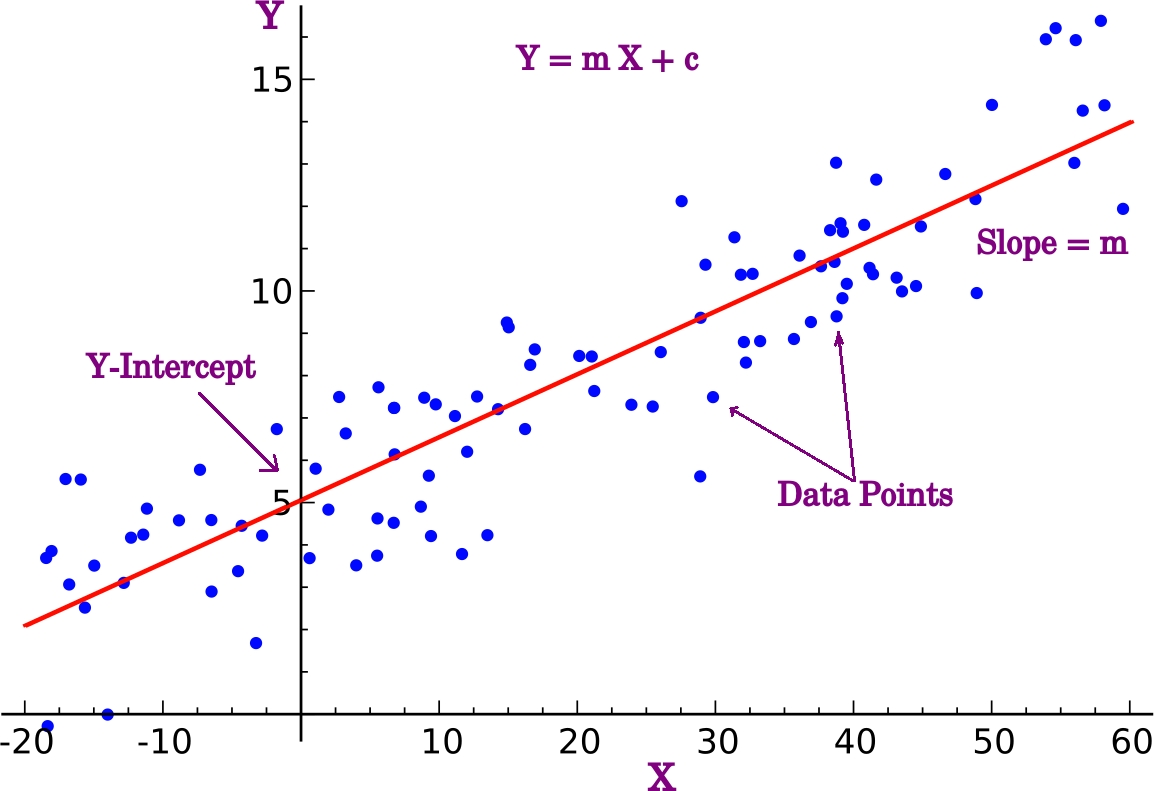
\includegraphics[width=0.8\linewidth]{figs/linear_regression.jpeg}
\end{figure}

The ultimate purpose is the find the best line (i.e. the best fit) between X and Y.\\
It should be mentioned that when we have multi-independent variables, the regression is then called \textit{Multiple Linear Regression}.\\
As a rule of thumb, if the correlation coefficient is reasonably large (positive or negative), the next step would be to fit the regression line which best models the data in order to help to make prediction on $Y$ given $X$.
\end{itemize}

\begin{itemize}
\item \textbf{$R^2$ Coefficient}: Related to Linear Regression, it is a coefficient of determination which reflects the fit goodness of the Line:
$$Variance_{~Y_{actual}} \times R^2 = Variance_{~Y_{predicted}}$$

So intuitively, the more $R^2$ is closer to 1, the more Actual Y and Predicted Y have {\color{blue}same variance} (i.e. same spread). That is the {\color{blue}actual variance is fully \textit{explained}} by the regression line.

We prefer $R^2$ over the correlation coefficients because it can quantify a linear relationship that is more {\color{blue} complicated} than a \textit{straight line}  
\end{itemize}

\begin{itemize}
\item \textbf{Adjusted $R^2$}: Useful over $R^2$ because it decreases when we add more {\color{red} junk} data and only increases if we have {\color{blue}meaningful} (i.e. useful) data.
\end{itemize}

\begin{itemize}
\item \textbf{Principle Component Analysis - PCA}:
It is used mainly to reduce the dimensions of multi-variate data (i.e. data that has more than one feature). It calculates for the importance of the features by using the {\color{blue} Singular Value Decomposition (SVD)} as follows:
\begin{itemize}
\item First it {\color{blue} centers} all points around the origin, so the new mean will be zero (this shift won't ruin the relative relation between the points but it will make the calculations easier).
\item Then for each feature (i.e. dimension), it finds the {\color{blue} best fit} of a line made by {\color{blue} projecting} the points of that feature; the best line should {\color{blue} maximize the distances} from the projected points to the origin.
\item The line is called PCA1 for the first feature and PCA2 for the second and so on..
\item The {\color{blue} Unit Vector} on that line (unit vector has the same direction but its length is one) gives us what is known as {\color{blue} Eigen Vector} (a.k.a Singular Vector). This vector is the Eigen Vector of the {\color{blue} Covariance Matrix} and since Eigen Vector by definition doesn't rotate and only scaled if multiplied by a rotation matrix, and since the rotation matrix here is the Covariance Matrix of the features, the Eigen Vector will have the {\color{blue} most spread} of the feature points.
\begin{figure}[h!]
  \centering
  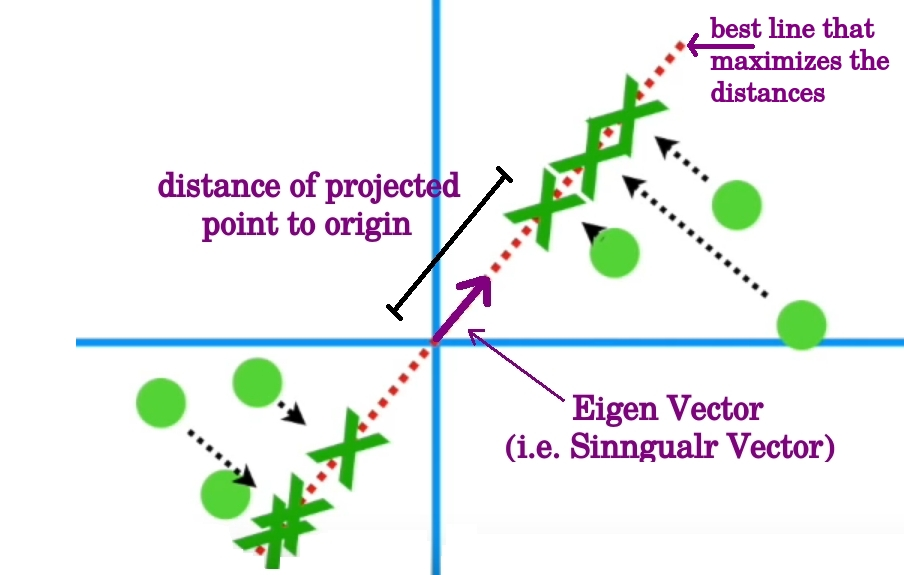
\includegraphics[width=0.75\linewidth]{figs/pca.jpeg}
\end{figure}
\item The cocktail recipe of how many we need from each feature according to the line and its slope called the {\color{blue} Linear Combination}.
\item The sum of the squared distances of the projected pointed on the line of each feature is called the {\color{blue} Eigen Values}, that's the {\color{blue} PCA score} (i.e. importance).
\item As a result, the PCA that has the {\color{blue} most variance} around, it is to be the {\color{blue} most important}.
\item To visualize PCA, check out {\color{blue} youtu.be/FgakZw6K1QQ}
\end{itemize}
\end{itemize}

\begin{itemize}
\item \textbf{Linear Discriminant Analysis - LDA}:
\begin{itemize}
\item PCA reduces the dimensions by focusing on the importance of the features (the feature with {\color{blue}most variation}).
\item LDA also reduces dimensions but it focuses on {\color{blue}maximizing the separation} among known categories.
\item It maximizes the distances between the means of the features and minimizes the variances of them.
\item Suppose we have two features, the purpose is:
$$\frac{(\mu_1 - \mu_2)^2}{\sigma_1^2 + \sigma_2^2} = \frac{ideally ~ large}{ideally ~ small}$$
\item LDA accounts for the most variation {\color{blue}between} categories.
\end{itemize}
\end{itemize}

\begin{itemize}
\item \textbf{Analysis of Variance - ANOVA}:
It is a statistical method to {\color{blue} compare the means} between two or more groups (like t-test but with a lot of groups / samples). ANOVA has different types, such as: 
\begin{itemize}
\item \textit{One-Way ANOVA}: one factor with at least two independent levels.
\item \textit{Repeated Measures ANOVA}: one factor with at least two dependent levels.
\item \textit{Factorial ANOVA}: two or more factors and levels can be either dependent or independent or both (mixed).
\end{itemize}
Assumptions on samples distribution:
\begin{itemize}
\item are normally distributed
\item independent of errors
\item no outliers
\item homogeneity of variance
\end{itemize}
ANOVA is useful to show the {\color{blue}interactions effects to test hypothesis}.
\end{itemize}

\section{Miscellaneous}
\begin{itemize}
\item \textbf{Standard Deviation v.s Standard Error}:
\centering
\begin{tabular}{|>{\centering\arraybackslash}m{3cm}|>{\centering\arraybackslash}m{4cm}|} 
 \hline
 $\sigma$ & std. error \\ 
 \hline
 How much the measurement spread out around the mean & The standard deviation of the mean (i.e. the mean of the means of many samples)  \\
 \hline
 Quantifies the variation within a set of measurements & Quantifies the variations in the means from multiple sets of measurements (tells how the mean is distributed) \\ 
 \hline
\end{tabular}
\end{itemize}

\begin{itemize}
\item \textbf{Bootstrap}:
Select a lot of samples randomly from original dataset allowing duplicates (i.e. with replacement) then calculate the mean of each sample.
\end{itemize}

\begin{itemize}
\item \textbf{Classification Performance Evaluation}:
Given the following abbreviations:
Number of True Positives, True Negatives, False Positives, False Negatives is TP, TN, FP, FN respectively, the most important metrics for evaluating classification performance are:

\begin{itemize}
\item \textbf{Sensitivity}:
$$Sensitivity = \frac{TP}{TP + FN}$$
Intuitively speaking, if we have a 100\% sensitive model, that means it {\color{blue}did not} miss any {\color{blue}TP}, in other words, there were {\color{blue}no FN}. However, here is a risk of having a lot of {\color{red}FP}.

\item \textbf{Specificity}:
$$Specificity = \frac{TN}{TN + FP}$$
Intuitively speaking, if we have 100\% specific model, that means it {\color{blue}did not} miss any {\color{blue}TN}, in other words, there were {\color{blue}no FP}, however, there is a risk of having a lot of {\color{red}FN}.

\item \textbf{Precision}:
$$Precision = \frac{TP}{TP + FP}$$
Intuitively speaking, if we have a 100\% precise model, that means it {\color{blue}could catch all TP} and there were {\color{blue}no FP}.

\item \textbf{Recall}: It is the \textit{Sensitivity}, but usually this term is used more by the Machine Learning Engineer whereas the Sensitivity term is more used by the Statisticians.\\
\begin{figure}[h!]
  \centering
  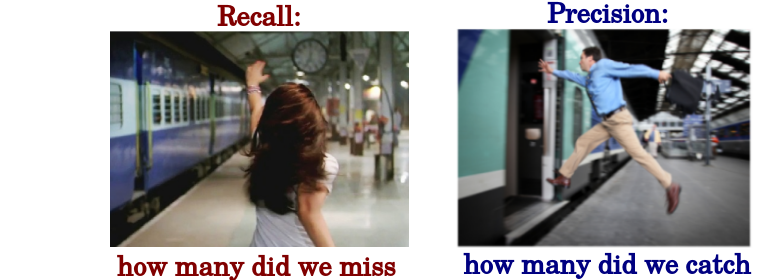
\includegraphics[width=0.9\linewidth]{figs/f1_score.png}
\end{figure}

\item \textbf{As a Rule of Thumb}:
if the cost of having FN is high, we want to increase the model {\color{blue}sensitivity} (i.e. recall).
For instance, in fraud detection or sick patient detection, we don't want to label/predict a fraudulent transaction (TP) as non-fraudulent (FN). Also, we don't want to label/predict a contagious sick patient (TP) as not sick (FN). 
That is because the {\color{red}consequences} will be worse than a False Positive (incorrectly labeling a a harmless transaction as fraudulent or a non-contagious patient as contagious).\\
On the other hand, if the cost of having FP is high, then we want to increase the model {\color{blue}specificity} and {\color{blue}precision}.
For instance, in email Spam detection, we don't want to label/predict a non-Spam email (TN) as Spam (FP). Whereas failing to label a Spam email as Spam (FN) is less catastrophic.

 
\item \textbf{F1 Score}: It's given by the following formula:
$$F_1~Score = 2 \times \frac{Precision \times Recall}{Precision + Recall}$$

F1 Score keeps a {\color{blue}balance} between Precision and Recall. We use it if there is {\color{red}uneven class distribution}, as precision and recall may give misleading results if used each one alone.
In other words, F1 Score is a comparison indicator between Precision and Recall Values.

\item \textbf{Area Under the Receiver Operating Characteristic Curve (AUROC)}:

It compares the {\color{blue}overall} (i.e. at different thresholds) Sensitivity vs (1-Specificity); that is the {\color{blue}True Positive Rate} vs {\color{red}False Positive Rate}.
Thus, the bigger the area under the curve, the greater the {\color{blue}distinction} between TP and TN.
\begin{figure}[h!]
  \centering
  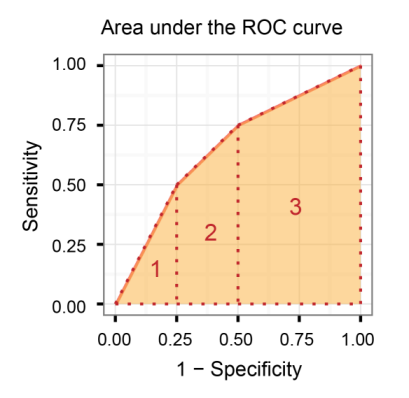
\includegraphics[width=0.7\linewidth]{figs/auroc.png}
\end{figure}


\item \textbf{AUROC vs F1 Score}:
In general, AUROC is for many different levels of thresholds and thus it shows the overall performance since it has many F1-score values. On the other hand, F1-score is applicable for any {\color{blue}particular point} on the AUROC.
You may think of it as a measure of precision and recall at a particular threshold value whereas AUROC is the whole area under the ROC curve, and for F1-score to be high, both precision and recall should be high.
{\color{blue}Consequently},  when you have a data {\color{red}imbalance} between positive and negative samples, you should always use F1-score because AUROC {\color{red}averages} over all possible thresholds.
\end{itemize}
\end{itemize}
\end{document}





